在 \Simulator\ 上模拟量子线路时，通常不需要考虑该量子线路是否真的能在量子芯片上执行；我们的关注点仅在于研究算法本身的可行性。然而，当考虑真实量子芯片时，芯片上可执行的量子门集合是有限的。此外，由于量子噪声的存在，我们也希望尽可能降低量子线路深度。因此，需要对量子线路进行编译和优化。本节将说明 \MindQuantum\ 如何完成量子线路的编译与优化。

这里，我们使用 DAG（Directed Acyclic Graph，有向无环图）作为量子线路编译工具。如图 \ref{fig:compiler} 所示，量子线路会被转换为 DAG。基于该 DAG，可以应用 \MindQuantum\ 中内置的编译规则，例如 \BasicDecompose、\FullyNeighborCanceler 和 \GateReplacer，以完成量子编译和优化。此外，我们还提供了两个稳健的管理器来组织这些编译规则，分别是 \SequentialCompiler 和 \KroneckerSeqCompiler。\SequentialCompiler 中的规则会按顺序各执行一次，而 \KroneckerSeqCompiler 中的规则会持续执行，直到无法进一步编译为止。

\begin{figure}
    \centering
    \begin{subfigure}{0.25\textwidth}
        \centering
        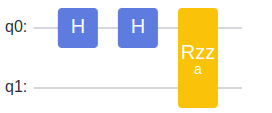
\includegraphics[width=\textwidth]{images/8_1_ori_circ.png}
        \caption{原始量子线路。}
        \label{fig:compiler_a}
    \end{subfigure}
    \begin{subfigure}{0.3\textwidth}
        \centering
        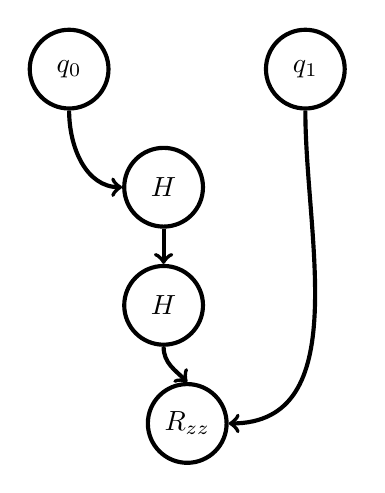
\begin{tikzpicture}[
                transparent/.style={circle, draw=black, fill=none, font=\sffamily, text centered, line width=1.5pt, minimum size=1cm}
            ]
            \node (q0) at (0, 0) [transparent] {$q_0$};
            \node (q1) at (3, 0) [transparent] {$q_1$};
            \node (H1) at (1.2, -1.5) [transparent] {$H$};
            \node (H2) at (1.2, -3) [transparent] {$H$};
            \node (Rzz) at (1.5, -4.5) [transparent] {$R_\text{zz}$};
            \draw [->, line width=1.5pt] (q0.south) to[out=270, in=180] (H1.west);
            \draw [->, line width=1.5pt] (H1.south) to[out=270, in=90] (H2.north);
            \draw [->, line width=1.5pt] (H2.south) to[out=270, in=135] (Rzz.north);
            \draw [->, line width=1.5pt] (q1.south) to[out=270, in=0] (Rzz.east);
        \end{tikzpicture}
        \caption{量子线路的 DAG 表示。}
    \end{subfigure}
    \begin{subfigure}{0.45\textwidth}
        \centering
        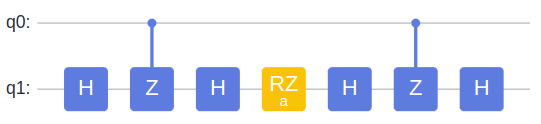
\includegraphics[width=\textwidth]{images/8_1_compiled_circ.png}
        \caption{编译和优化后的线路。}
        \label{fig:compiler_c}
    \end{subfigure}
    \caption{将量子线路转换为 DAG，并依据给定编译规则完成编译。}
    \label{fig:compiler}
\end{figure}

作为示例，我们将使用不同规则来编译并优化图 \ref{fig:compiler_a} 中的线路。首先，使用 \BasicDecompose 和 \FullyNeighborCanceler 构建一个 \KroneckerSeqCompiler，以便将 $R_\text{zz}$ 门分解为基础量子门，并抵消两个 Hadamard 门。接下来，假设芯片只能执行 CZ 门，则将 CNOT 门替换为 CZ 门。
\begin{lstlisting}
from mindquantum.core.circuit import Circuit
from mindquantum.algorithm.compiler import *

circ = Circuit().h(0).h(0).rzz('a', [0, 1])

compiler = SequentialCompiler([
    KroneckerSeqCompiler([
        BasicDecompose(),
        FullyNeighborCanceler()
    ]),
    CXToCZ()
])

new_circ = compile_circuit(compiler, circ)
\end{lstlisting}
